\section{Introduction}
\label{sec:intro}

\begin{figure}[!t]
  \centering
  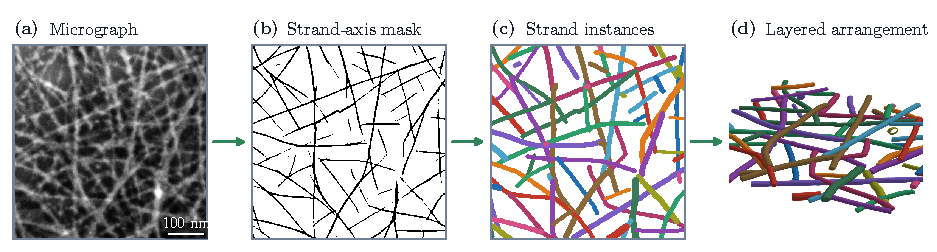
\includegraphics[width=\linewidth]{figures/fig_graphical_abstract.pdf}
  \caption{From micrograph to individual strands, on one carbon-nanotube SEM
    field held out of the segmenter's training data. \textbf{(a)} A fixed
    central crop. \textbf{(b)} The strand-axis mask from the upstream
    segmenter. \textbf{(c)} The instances PLECTA reconstructs from that mask
    alone, each drawn at the width measured for it across its own centreline.
    \textbf{(d)} The layered arrangement estimated for the same instances, at
    the same widths and without vertical exaggeration. Colour carries instance
    identity in both (c) and (d) and nothing else.}
  \label{fig:graphical-abstract}
\end{figure}

The effective properties of a strand network are influenced by the arrangement
of its individual strands, but a micrograph shows those strands only as an
overlapping tangle. This paper recovers them as separate objects from a single
greyscale scanning electron micrograph, and estimates which strand lies on top
at each crossing, placing them in depth
(Figure~\ref{fig:graphical-abstract}). The problem is not specific to one
material.

Many materials comprise networks of long, overlapping strands, including
carbon-nanotube (CNT) sheets, collagen in connective tissue, paper and nonwoven
textiles. Their stiffness, strength and conductivity depend on network
geometry, constituent behaviour and inter-strand interactions. For example,
load transfer between nanotubes can limit an assembly's stiffness and strength
despite the high modulus of each tube. Predictive models therefore require
geometric inputs such as strand length, orientation, curvature and
connectivity. Bulk image measurements such as coverage and orientation do not
establish which visible segments belong to the same strand. Recovering that
identity is necessary to measure individual strands end to end.

This is an instance-segmentation problem in which the objects are long, open
curves that overlap one another. Crossings merge distinct strands into one mask
component, whereas signal gaps split one strand into fragments whose tips can
be indistinguishable from genuine ends. Reconstruction must therefore decide
which segments continue through each junction and which reconnect across a
gap. Section~\ref{sec:related} reviews existing approaches, with the
corresponding references, and their relation to the present work.

We approach this in two steps. A greyscale micrograph is first reduced to a
binary mask marking the strand axes, by a segmenter trained on synthetic image
and mask pairs, so that no micrograph has to be annotated by hand. That mask
records where the network lies, but not which segments belong to the same
strand. Here, we address the step that follows: recovering the individual
strands from that mask alone, while allowing genuine ends, reconnecting gaps
and leaving each crossing to every strand that runs through it.

PLECTA does this by jointly selecting pairs of arms, the strand
segments entering a junction, while allowing arms to remain unpaired. It
solves an exact maximum-weight \emph{partial}-matching problem at each junction,
with an explicit penalty for unmatched arms and no restriction on junction
degree. It combines this decision with geometric checks for reconnecting gaps
and updates to direction and curvature estimates as longer strands are
assembled.
Reconstruction is deterministic for fixed inputs and parameters and assumes
directional continuity, targeting semiflexible networks whose strands maintain
their direction locally through crossings.

We evaluate PLECTA on synthetic scenes and annotated scanning electron
microscopy (SEM) images of CNT sheets, using paired clean and degraded masks
to isolate the effect of mask quality. Across the evaluated datasets, PLECTA
reconstructed strand identity more accurately than the compared methods,
although performance remained sensitive to network density and mask quality.
For SEM images, an upstream segmenter supplies the strand-axis masks. A
separate stage uses the corresponding greyscale image to estimate which strand
lies on top at each crossing; this is a proof of concept for depth ordering,
not a validated three-dimensional reconstruction.
Section~\ref{sec:methods} describes the workflow and evaluation,
Section~\ref{sec:results} reports the results, and
Section~\ref{sec:conclusions} discusses conclusions and limitations.
\Igor{After this intro, i still do not have clear image on what is the contribution of the paper. "Combination of ingridients" does not sound good. Maybe some early image -- not necessarily exhaustive, but simple and schematic -- could help.}
